\documentclass[11pt, oneside]{article}
\usepackage{graphicx}
\usepackage{url}
\begin{document}

\title{The Second Screen}
\author{Michael Fraser}
\maketitle

\begin{abstract}
For this topic, 
you are asked to investigate the history of second 
screen technologies and to place the latest such 
offerings in the context of this history
\end{abstract}

\tableofcontents

\section{Introduction}
Almost everyone these days has a tablet or smart phone device. As the various forms of media begin to recognize this face, they begin to utilize it to their advantage. It used to be that people would sit down and watch TV with whatever TV screen they had at the time, and interaction with their favorite TV shows was limited to this action. As technology advanced, the common TV watcher was granted easy accessibility to a second screen of sorts: a tablet or smart phone. 

The same is true for users of entertainment systems and computers; multiple screens are available to push the limits of interaction with common devices. Applications and devices are now able to allow for a more in-depth interaction with the systems people have interacted with in a limited way for so long. Are these so called "second screens" going to replace the traditional forms of interaction with common systems, or will it remain a specialized tool for specific applications?

\section{Background}

\subsection{Computers}
Computers have had the capability to connect to multiple screens since the late 90's. As computers have advanced technologically though, applications for a second monitor have stayed relatively the same. Multiple monitors provide the user with a larger space to spread around programs and applications. It is possible to connect together many monitors, as can be seen in Figure \ref{monitors}. Multiple monitors do not follow with the second screen ideology, as multiple monitors are mostly used as a single, larger screen rather than two separate systems. Computers can still be part of second screen systems though, as the computer could interact with a phone, tablet, or even a TV. 

\begin{figure}[h!]
    \centering
    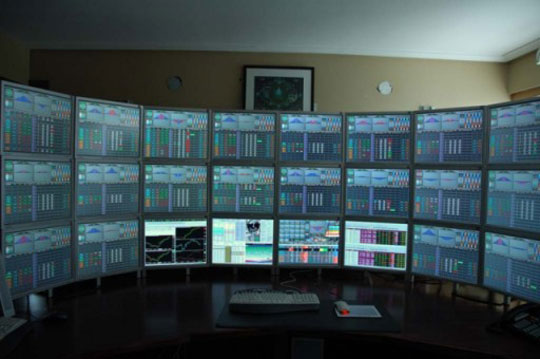
\includegraphics[width=.8\textwidth]{Multiple-Monitor-Setup.jpg}
    \caption{An example of utilizing multiple monitors.}
    \label{monitors}
\end{figure}

\subsection{Entertainment Systems}
A second screen application can also be found with the top entertainment systems as well. Systems as early as the Dreamcast were making use of a second screen to add more interaction between the user and the games they play. With the Visual Memory Unit (VMU), Dreamcast users could download mini-games that could be played separately and later incorporated back into the game. The GameCube was the next to utilize a second screen by allowing users to connect a Game Boy Advance to the console. By connecting the two games, the user could share file information or items and have it directly affect the two games being connected.

The Wii U was released to work alongside the Wii to allow users a second screen to utilize while playing their favorite game. The Wii U controller had the second screen that allowed users to perform secondary tasks, such as select something from inventory or view a map. Soon after, Microsoft unveiled the Xbox SmartGlass, designed to work with the Xbox 360 to allow easier interaction with the console. Instead of producing a new device for the second screen, Microsoft utilized the technology that users already have: their smartphones and tablets. The Xbox SmartGlass is an app for the Iphones, Android phones and tablets, and Windows 8 devices \cite{MashableSmartGlass}.

Table \ref{entertainment_table} shows a list of primary and secondary screens that entertainment systems have used to increase interactivity with video games. 

%Not sure why this does not center more properly..
\begin{table}[h!]
    \centering
    \caption{List of primary and secondary screens for entertainment systems \cite{wiki_second_screen}.}
    \begin{tabular}{| c | c |}
        \hline
        Primary Screen & Second Screen \\ \hline
        Dreamcast & VMU \\ \hline
        GameCube & Game Boy Advance \\ \hline
        PlayStation 3 & Playstation Portable and PlayStation Vita using Remote Play \\ \hline
        Playstation 4 & Playstation Vita using Remote Play; iOS, Android using PlayStation App \\ \hline
        Wii & Nintendo DS \\ \hline
        Wii U & Wii U GamePad and Nintendo 3DS \\ \hline
        Xbox 360 & Windows 8, Windows Phone, iOS, Android using Xbox SmartGlass \\ \hline
        Xbox One & Windows 8, Windows Phone, iOS, Android using Xbox SmartGlass \\ \hline
    \end{tabular}
    \label{entertainment_table}
\end{table}

\subsection{Television} % ------------- Need to edit this
Second screen development is most common with televisions, where tablets or smart phones are used to connect users to their shows in an alternative way. The users view the programs and use their second screens to answer questions or find out more details about a particular scene. Figure \ref{second-screen} shows a tablet displaying the same program as the TV. Since the development of social networking sites like Facebook and Twiter, the media has been engaging their supporters through mass messages. Prime time shows like Covert Affairs post statuses on the show's facebook page engaging followers about the decisions made in the show, whereas shows like Tosh.0 have the host direct the viewers into tweeting about things Tosh has said. 

\begin{figure}[h!]
    \centering
    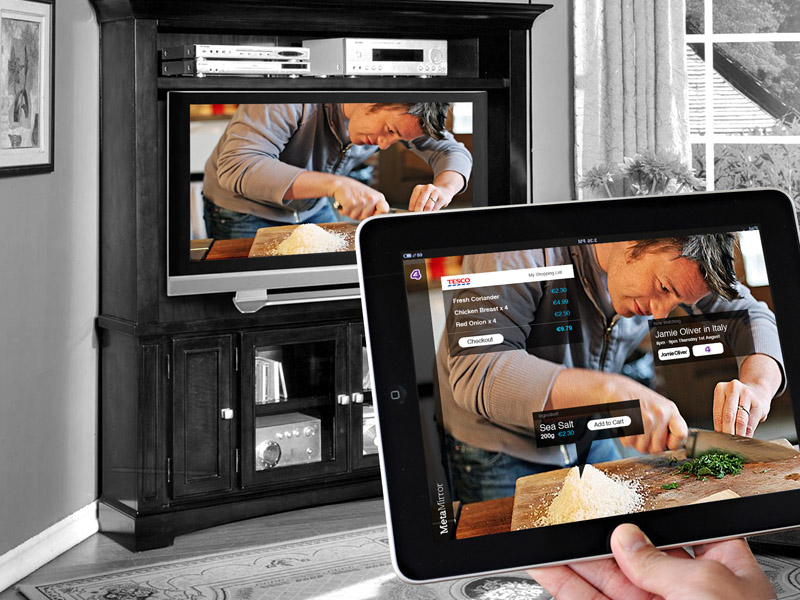
\includegraphics[width=.8\textwidth]{second-screen.jpg}
    \caption{Example of the second screen with respect to TV (advanced-television.com).}
    \label{second-screen}
\end{figure}

Studies completed by Twitter have found that when a show is airing that directly integrates tweets into the content, there is a major increase in the number of tweets engaging the show's hashtag subjects \cite{TwitterTV}. Chris Gorham of Covert Affairs was interviewed by Mashable on the effects of the second screen and the show's success. He believes Twitter is a way of sharing the behind-the-scenes process with his fans \cite{MashableChris}. 

The usefulness of a second screen was tested with a subtitle and sign-language system, where subtitles or sign language corresponding to what is watched on TV was produced on the second screen \cite{IEEE_EFS}. While the program provided the sign language and subtitles for the viewed program, it was found that syncing the TV screen and second screen TV was difficult. An illustration of how the second screen provided sign language for a program can be found in Figure \ref{sign-language}.

\begin{figure}[h!]
    \centering
    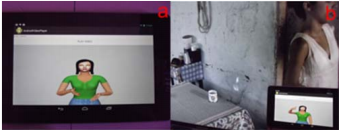
\includegraphics[width=.8\textwidth]{SignLanguage.png}
    \caption{Example of how a second screen can be used to improve the viewability of TV \cite{IEEE_EFS}.}
    \label{sign-language}
\end{figure}

While social networking provides the means for interaction with shows, the audiences are actually creating 

\section{Methods}
A simple Google search reveals that this is not a new concept. Hundreds of articles or blog posts can be found on the topic of second screen, all revolving around the TV and media. To investigate whether or not the second screen was here to stay, searches were done in the IEEE Xplore digital library along with simple web searches. IEEE Xplore provided an article involving a more technical application of the second screen, whereas simple web searches provided blogs on how the media and social networking use second screens as a way to engage viewers at home. 

\section{Discussion}
Whether it is a facebook status asking followers about a certain moment of a show or the host of a show telling viewers to tweet what they think, social networking is a big part of the second screen movement. 

\section{Conclusions}
Conclusions

\bibliography{mental.bib}{}
\bibliographystyle{plain}

\end{document}
